\chapter{مقدمه}
\section{مقدمه}
رایانش ابری\LTRfootnote{Cloud Computing} یکی از حوزه‌های در حال تحول کامپیوتر است که به یک جنبه‌ی حیاتی از فناوری و مشاغل مدرن تبدیل شده است. این الگو همچون انقلابی، شیوه‌ی ارائه و مصرف منابع محاسباتی را متحول کرده است و فرصت‌های جدیدی را برای سازمان‌ها فراهم کرده تا کارایی و رقابت خود را بهبود بخشند. یکی از پایه‌ای‌ترین و رایج‌ترین شکل‌های رایانش ابری، زیرساخت به عنوان خدمت (\lr{IaaS})\LTRfootnote{Infrastructure As A Service} است که منابع محاسباتی مجازی مانند فضای ذخیره‌سازی، قدرت پردازش و پهنای باند را از طریق اینترنت در اختیار کاربران قرار می‌دهد\cite{Mell_2011}.

\begin{figure}[h]
	\vspace{1cm}
	\centering
	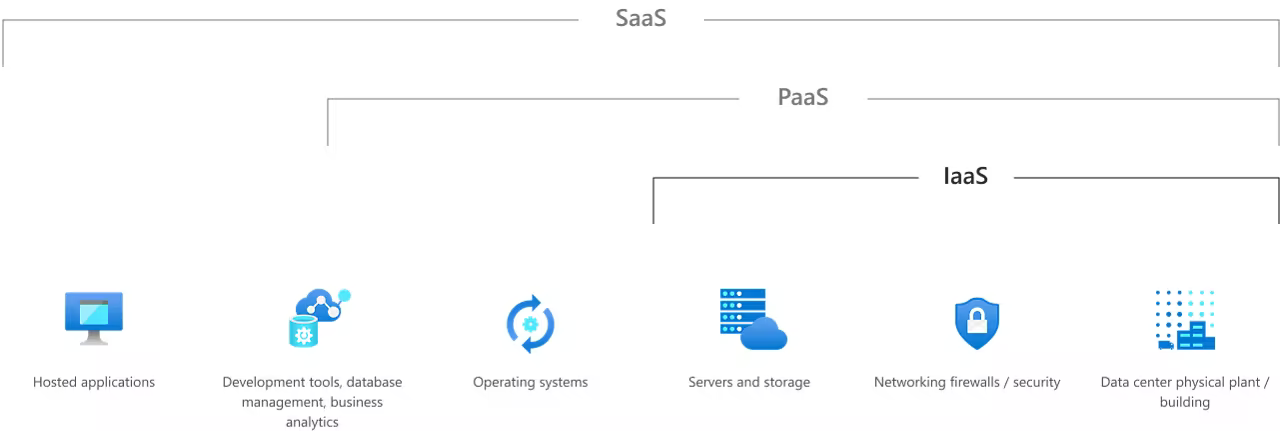
\includegraphics[scale=0.35]{figures/cloud_computing_models.png}
	\caption{انواع مدل‌های رایانش ابری\cite{microsoft_cc_models}}
	\label{fig:cc_models}
\end{figure}

این الگو را از دو دیدگاه می‌توان بررسی کرد. دیدگاه اول مختص کاربران مصرف‌کننده است که برای استفاده و مصرف منابع دیگر دغدغه‌ای نسبت به زیرساخت استفاده شده برای ارائه‌ی خدمات ندارند. دیدگاه دوم مربوط به ارائه دهندگان این خدمت است. از این دیدگاه، توسعه یک سکو\LTRfootnote{Platform} کارآمد و قابل اعتماد که بتواند مشتریان را جذب و حفظ کند، بسیار مهم است. از این رو، شرکت‌ها و توسعه‌دهندگان سراسر دنیا همواره سعی در توسعه و فراهم‌کردن ابزارها با این هدف دارند. یکی از معروف‌ترین این شرکت‌ها، شرکت \lr{VMWare} است که برنامه‌های فراوانی برای فراهم کردن زیرساخت ارائه‌ی خدمات ابری توسعه داده است. چالش بعدی ارائه‌دهندگان، فراهم کردن و طراحی یک رابط برنامه‌نویسی (\lr{API})\LTRfootnote{Application Programming Interface} است که بتواند با مشتریان و ارائه دهنده زیرساخ\LTRfootnote{Infrastructure Provider} تعامل داشته‌باشد و آن‌ها را قادر سازد منابع مجازی خود را مدیریت کنند.
\section{تعریف مسئله}
در این پروژه قصد داریم که خدمات جامع یک ارائه‌دهنده‌ی زیرساخت به عنوان خدمت را که بر بستر ابزار \LTRfootnote{https://vmware.com/products/cloud-director.html}\lr{VMWare Cloud Director} فراهم شده است را توسط یک رابط برنامه‌نویسی به کاربران ارائه دهیم. برای این هدف، باید خدمات کاربردی، مدیریتی، نظارتی و امنیتی را در یک لایه‌ی جدا تعریف کنیم و این لایه از برنامه‌ی خود را با ابزار زیرساختی در تعامل نگه داریم. 
\section{راه حل پیشنهادی}
برای توسعه این محصول، بایستی در ابتدا با بررسی نیازمندی‌ها و محدودیت‌های زیرساخت و کاربران، اقدام به طراحی کلی سامانه کرد. با توجه به گسترده بودن این نیازمندی‌ها و توسعه‌پذیری جداگانه آن‌ها، باید طراحی کلی این سامانه به صورت پیمانه‌ای\LTRfootnote{Modular} و با کمترین وابستگی میان واحد‌ها باشد. در این گزارش، ابتدا به طراحی و شرح قسمت‌های مختلف سامانه می‌پردازیم و سپس جزئیات فنی هر قسمت و تعامل قسمت‌ها را بررسی می‌کنیم.


هدف ما، پیاده‌سازی یک سامانه‌ی کاربردی کامل است که با استفاده از رابط برنامه‌نویسی تحت وب، بتوانیم خدمات را از آن دریافت کنیم. این خدمات شامل موارد زیر است.

\begin{enumerate}
	\item \textbf{احراز هویت}
	
	\item \textbf{خدمات ابری}
	
	\item \textbf{مدیریت و حسابداری}
\end{enumerate}

این خدمات باید با دسترسی‌پذیری بالا\LTRfootnote{Highly Available} و به صورت توزیع‌شده\LTRfootnote{Distributed} توسعه پیدا کنند که پاسخگوی نیازمندی‌های کاربران در شرایط خاص و فشار‌های بسیار بالا باشد.

\subsection{احراز هویت}
هدف از پیاده‌سازی این قسمت، ایجاد سطوح دسترسی مختلف برای کاربران و کنترل دسترسی کاربران به منابع است. در این سامانه، کاربران انتظار خدمات زیر در حوزه‌ی احراز هویت را دارند.

\begin{itemize}
\item \textbf{ایجاد حساب کاربری}: کاربر سامانه باید بتواند با نام کاربری و کلمه عبور، اقدام به ساخت حساب کاربری نماید. پس از ساخته‌شدن این حساب، دسترسی به منابع فقط با داشتن این اطلاعات هویتی امکان‌پذیر است.

\item \textbf{سطوح دسترسی مختلف}: با توجه به گستردگی خدمات ارائه‌شده، سطوح دسترسی متفاوتی باید داخل سامانه قابل تعریف باشد.

\item \textbf{مدیریت دسترسی}: مدیر سامانه باید بتواند موقتاً یا دائماً دسترسی کاربران را از سامانه بگیرد.

\item \textbf{صحت‌سنجی درخواست‌ها}: پس از احراز هویت کاربر، تمامی درخواست‌های ورودی به سامانه باید صحت‌سنجی شوند.
\end{itemize}

\subsection{خدمات ابری}
کاربرد اصلی این سامانه، ارائه خدمات \lr{IaaS} در بستر یک رابط برنامه‌نویسی تحت وب است. این خدمات با تمرکز بر ارائه‌ی ماشین‌های مجازی و عملیات قابل تعریف بر روی آن شامل موارد زیر است.

\begin{itemize}
	\item ساخت ماشین مجازی
	\item حذف ماشین مجازی
	\item ویرایش مشخصات ماشین مجازی
	\item ساخت \lr{Image} و برنامه‌های قابل اجرا روی ماشین مجازی
	\item حذف و ویرایش برنامه‌های قابل اجرا روی ماشین مجازی
	\item ارسال دستورات روشن، خاموش، راه‌اندازی مجدد به ماشین‌های مجازی
	\item ارسال دستور تهیه نسخه‌های پشتیبان از ماشین مجازی
	\item تعریف شبکه‌های محلی
	\item تعریف شبکه‌های خصوصی
	\item اضافه کردن ماشین مجازی به یک شبکه
\end{itemize}

\subsection{مدیریت و حسابداری}
دسته‌ی دیگری از خدمات که علاوه بر کاربران، برای مدیر سامانه نیز تعریف می‌شود، عملیات مربوط به مدیریت، نظارت و حسابداری است. لیست این عملیات به شرح زیر است.

\begin{itemize}
	\item تعریف سهمیه‌ی\LTRfootnote{Quota} منابع
	\item حذف سهمیه‌ی منابع
	\item بروزرسانی استفاده از سهمیه
	\item رصد کردن مصرف منابع
	\item دریافت گزارش از مصرف منابع
	\item تعریف اعتبار مالی
	\item تعریف هزینه‌های منابع
	\item اعتبارسنجی درخواست‌ها با توجه به سهمیه و اعتبار
\end{itemize}

\subsection{قابلیت‌های غیرعملکردی}
علاوه بر نیازمندی‌ها و قابلیت‌های عملکردی که در بخش‌های گذشته مطرح شد، دسته دیگری از نیازمندی‌ها و قابلیت‌ها وجود دارد که جنبه‌ی غیرعملکردی دارند. این قابلیت‌ها مربوط به اجرا،امنیت، نگهداری و توسعه سامانه می‌شود.

در اجرای سامانه، باید به این نکته که بار سامانه بسته به تعداد کاربران و نوع درخواست‌ها تغییر می‌کند توجه داشت و تمهیدات لازم جهت اجرای مناسب برنامه در سناریو‌های مختلف را تدارک دید. از جمله این تمهیدات، مقیاس کردن برنامه متناسب با بار، اجرای مجدد سامانه در صورت بروز خطا، تقسیم درخواست‌ها است.

گروه دیگری از قابلیت‌ها، مربوط به امنیت سامانه است. هدف از این قابلیت‌ها، شناسایی زودهنگام آسیب‌پذیری‌های ممکن و رفع آن‌ها در جهت بهبود امنیت سامانه در اجرای نهایی است. از جمله این قابلیت‌ها، سازوکارهای مقاوت بر آسیب‌پذیری‌های پایگاه داده، جلوگیری و کاهش اثر حمله‌های شبکه‌ای است.

دسته‌ی آخر از قابلیت‌های غیر عملکردی، شامل امور نگهداری و توسعه سامانه است. از میان این قابلیت‌ها، ثبت وقایع به شیوه‌ی موثر و مناسب، ذخیره معیار\LTRfootnote{Metric}‌های مختلف برنامه، پیاده‌سازی داشبوردهای نظارتی از کلیدی‌ترین نیازمندی‌‌های سامانه هستند.

در ادامه، جزئیات فنی و ابزار‌های مورد استفاده جهت ارائه این قابلیت‌ها توضیح داده شده‌است.


\section{کارهای مشابه}
با توجه به محبوبیت رایانش ابری و خدمات ارائه زیرساخت، اکثر قریب به اتفاق شرکت‌های فعال در این حوزه اقدام به ارائه درگاه‌های ارائه خدمات ابری به صورت رابط برنامه‌نویسی کرده اند که در ادامه با این محصولات آشنا می‌شویم.

\subsection{نمونه‌های داخلی}
از بین شرکت‌های داخلی فعال در این حوزه، شرکت ابرآروان اقدام به ارائه‌ی خدمات \lr{IaaS} در قالب رابط ارتباطی تحت وب کرده است.

این رابط که در این آدرس\cite{arvancloud} تفسیر شده است، تمامی خدمات قابل تعریف برروی ماشین مجازی و منابع مجازی را مشخص کرده. با توجه به متن‌بسته بودن این سرویس، نمی‌توان بیش از این در مورد معماری و جزئیات پیاده‌سازی خدماتی که ارائه می‌شود، صحبت کرد.


یکی دیگر از شرکت‌های ارائه دهنده خدمات مشابه، شرکت آسیاتک است. مستندات مربوط به عملکرد سرویس ارائه خدمات ابری این شرکت، در این آدرس\cite{asiatech} قرارداده شده‌است.


\subsection{نمونه‌های خارجی}
شرکت‌های بزرگ فعال در حوزه‌ی خدمات ابری نظیر گوگل، مایکروسافت، آمازون، دیجیتال اوشن، اوراکل و آی‌بی‌ام، همگی سرویس ارائه‌ی خدمات \lr{IaaS} را به صورت عمومی برای استفاده کاربران فراهم کرده‌اند. معماری و نحوه‌ی سرویس‌دهی تمامی این ارائه دهندگان به شکل مشابه و بر مبانی الگوی پرداخت بر اساس مصرف\LTRfootnote{Pay-As-You-Go} است. منتها به دلیل متن‌بسته بودن این سرویس‌ها، اطلاعات بیشتری در مورد جزئیات پیاده‌سازی آن‌ها در دسترس نیست. با این وجود، با بررسی دقیق‌تر و جزئی‌تر مستندات سرویس‌ها می‌توان کلیاتی در مورد طراحی و عملکرد سامانه‌ها به دست آورد که در فصل بعد به بررسی این موارد می‌پردازیم.